\documentclass[a4paper]{article}

\usepackage{amsmath}
\usepackage{amsfonts}
\usepackage{graphicx}
\usepackage{enumerate}
\usepackage{SIunits}
\usepackage{hyperref}
\usepackage{anysize}
\usepackage{hyperref}

\marginsize{2.5cm}{2.5cm}{1.5cm}{1.5cm}

\graphicspath{{./images/}}

\title{Design of Digital Platforms}
\author{Steven Janssens, Pieter Maene en Kristof Mari\"en}
\date{\today}

\begin{document}
\maketitle

\section{Overall Architecture}

After having written a software implementation of the Montgomery algorithm in \textit{C}, the conclusion was that this was too slow for a real implementation. Therefore, in the second part of this course, we had to build a hardware coprocessor that should significantly increase speed. The final goal of this project was to build RSA encryption and decryption.\\

\begin{figure}[h]
	\center{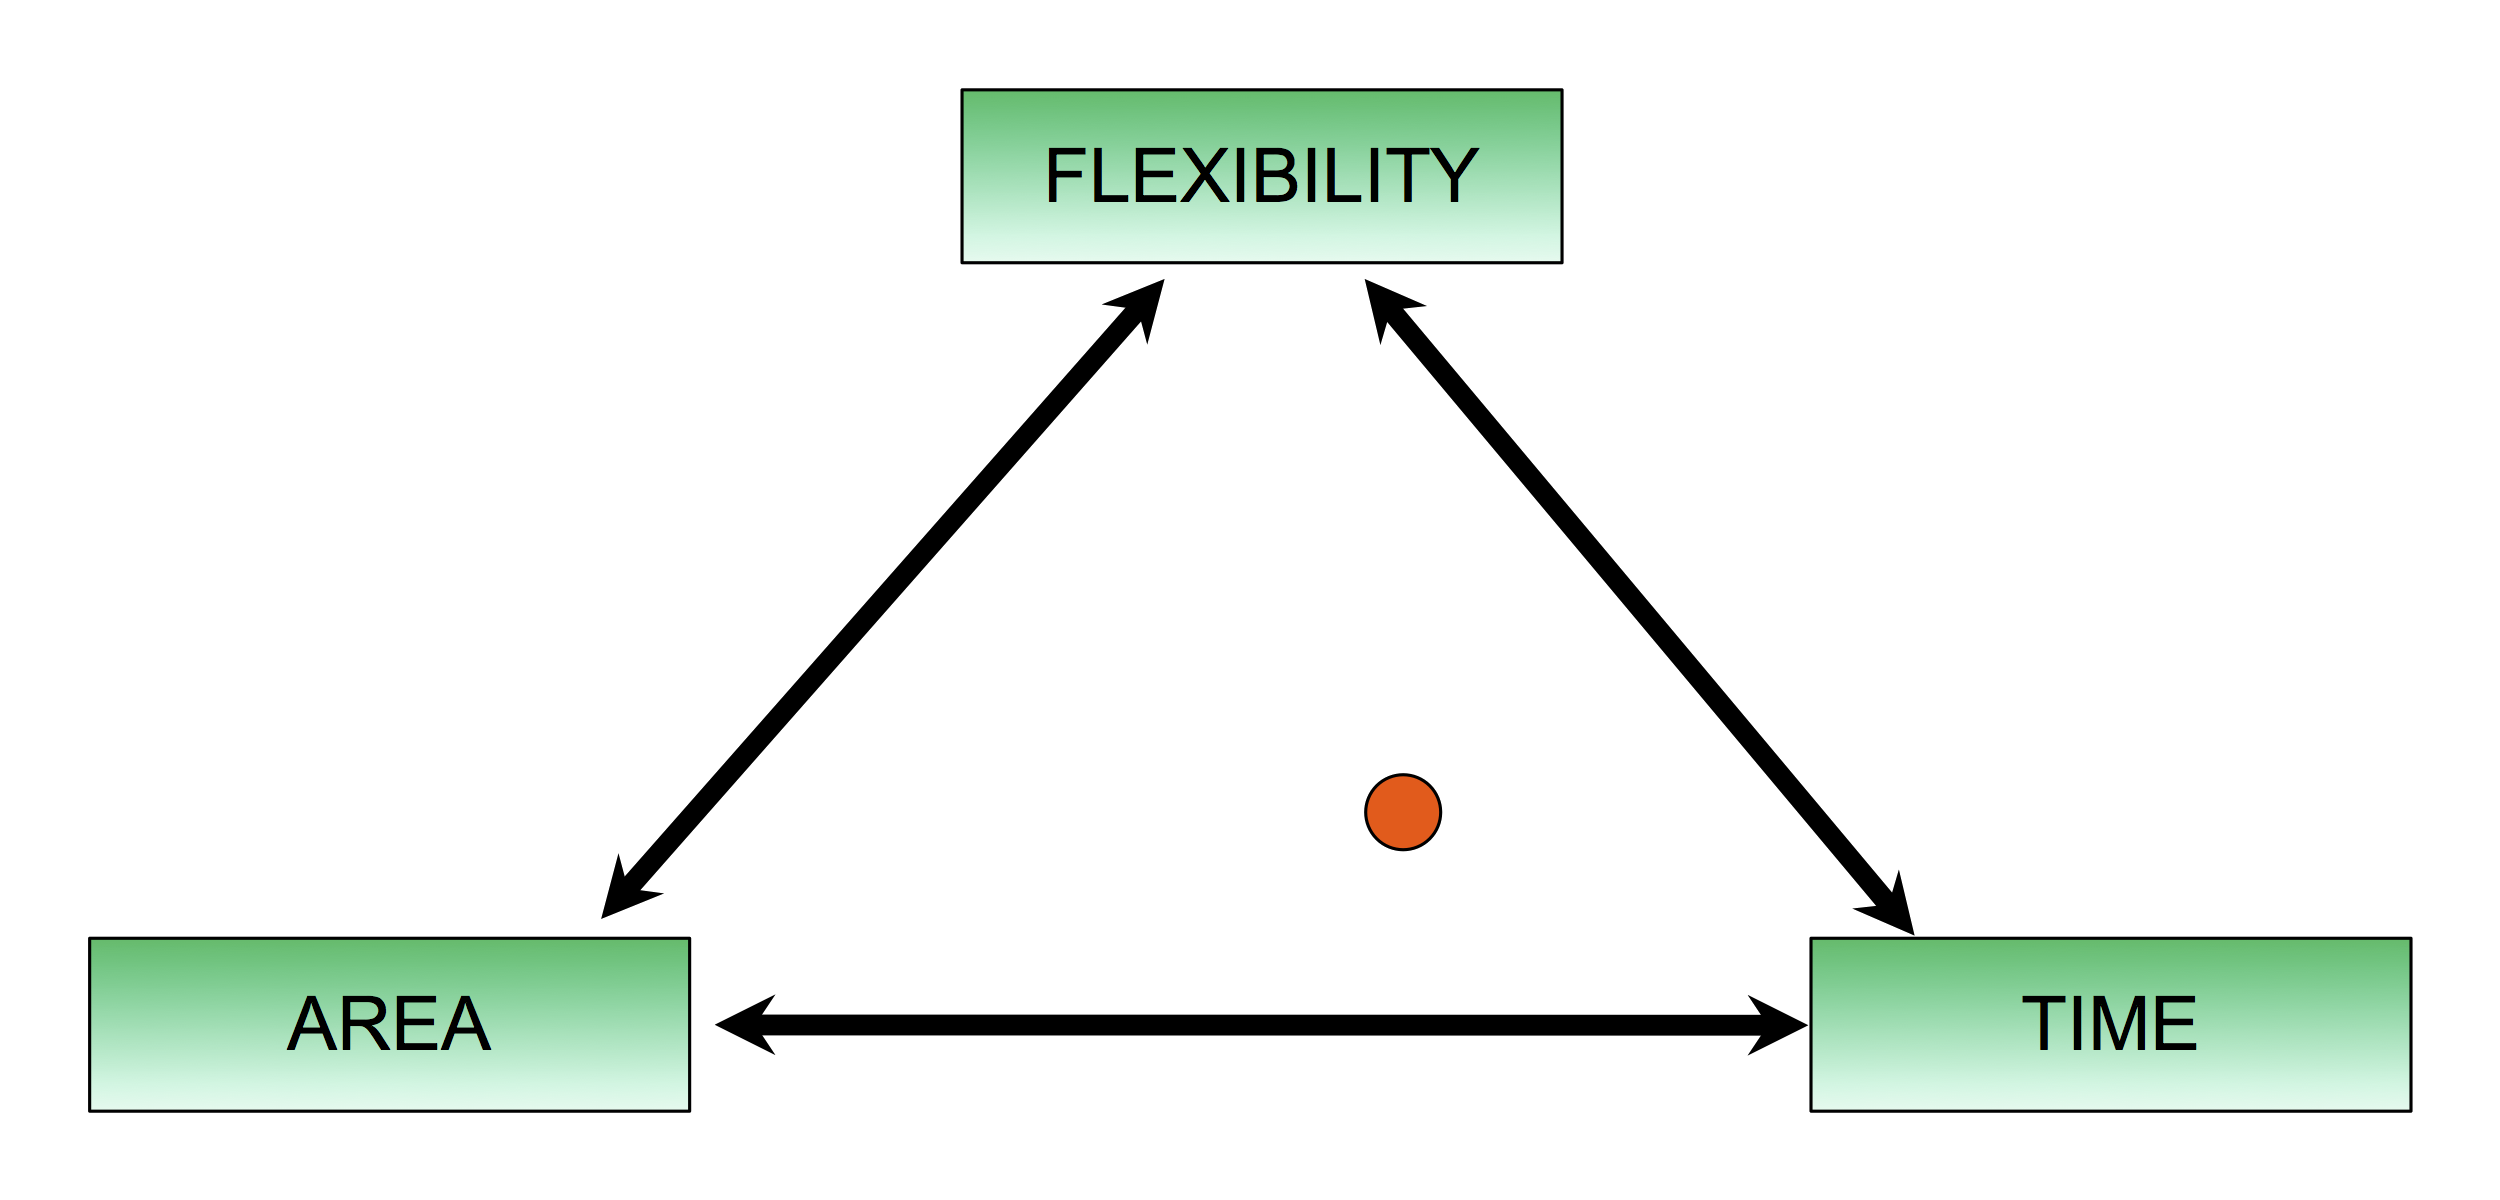
\includegraphics[width=0.8\linewidth]{situation.png}}
	\caption{Situation}
	\label{fig:situation}
\end{figure}

\section{HW/SW Boundaries}

The RSA algorithm is a basic and very often used algorithm for encryption and decryption of data. So it is important that the encryption and decryption is as fast as possible. The algorithm is standardized and will not change in the future. The only part of it that will change is the size of the inputs. Because of these facts we have chosen for a full hardware implementation.\\

From the previous section we know that a Montgomery multiplication takes about 1 second and a Montgomery exponentiation uses a lot of multiplications. So the multiplication must be done in hardware. Our hardware implementation takes about 1300 cycles. Assuming a clock frequency of about 5 \mega \hertz, this means a multiplication in hardware takes about 0,26 \micro \second.\\

So the only choice that was left, was to do the exponentiation in \textit{C} and call every time the Montgomery multiplication of the hardware. But doing this would cause a lot of overhead to transfer the data from the software to the hardware en back. So we decided to write the exponentation in \textit{Gezel} as well.

\section{HW/SW Interface}

\section{Performance Metrics}

\section{Synthesis Results}

\section{Test Strategy}

Since the RSA algorithm is a quite complex one, a test strategy has to be used. Otherwise it will be very difficult to see where errors occur. Because our code is completely implemented in hardware, the only possibility to give an output is by using display-statements. Further it can be easy to use finish statements in the \textit{Gezel} code to stop the simulation of the hardware immediately. However, this sfg will be only used once and sometimes this is not a possibility because the result only comes out after a few iterations. This problem can be solved by using a seperate sfg that is used when the result is completed or by using the same display statement in the cycle after the result is ready. But the first thing to test, is whether the inputs are correct. If the values given from the software are not matching the data in the hardware, the result will be quite random and the right result will never be given. Afterwards, the algoritm itself can be debugged.\\

The RSA algorithm mainly consists of a Montgomery exponentiation, which repeatedly computes Montgomery multiplications. By splitting the complex problem up into small problems, it is also easier to test. So first the Montgomery multiplication will be tested by using several testvectors and see whether the multiplication is correct. It is best to work with small vectors of 8 bit for instance, because then it is easier to go through all individual steps and errors can be found easier. When the multiplication works for small numbers, it can also be tested on big numbers. If this works properly, the higher complexity of the Montgomery exponentiation can be tested. And finally, the encryption and decryption can be tested in serial by first doing the encryption on the given message and afterwards performing the decryption on this ciphertext. If the result of this decryption is exactly the message originally sent, the RSA algorithm works properly.\\

For debugging the exponentiation, after checking the correctness of the inputs, the first Montgomery multiplication for \tilde{x} will also displayed. Only if this value is equal to the value coming out of the Magma calculator, the further debugging can begin. For easier debugging, the whole exponentiation algorithm was implemented in \textit{Maple}. So each step could be analysized and errors could be seen quicker. To measure the amount of iterations, a display of the counter can be used. This counter begins at the maximum wanted iterations and decrements always by one before the next iteration is started. When the counter comes to zero, the loop must not be executed and the last Montgomery multiplication can be started. By using the \textit{Maple} file, the outcome of the for-loop is known and this can be controlled first. Afterwards, there is only one Montgomery multiplication left. The outcome of this multiplication is also the output of the Montgomery exponentiation. When using encryption, the ciphertext of the Magma calculator must be the result and for the decryption, the original message must be the result.\\

To check if the result of the encryption or decryption is well transfered to the software, the result has to be sent back to the hardware. Only here the display statements can be used. To control this connection between hardware and software, displays can be used to see which data is sent. When the complete result is transferred to the \textit{C} code, this result has to be read in back to the \textit{Gezel}, where it can be read.
\end{document}
